\chapter{Map Details}

\section{Schematic Map Representation}
We have internally divided our map area into a grid of 20 by 20. Consider the schematic diagram of our map in Figure 2. We have represented the map details for one team in a table. The other team area has been left blank for it is a copy and paste mirror image of the same around the diagonal.

\begin{figure}[htp]
\centering
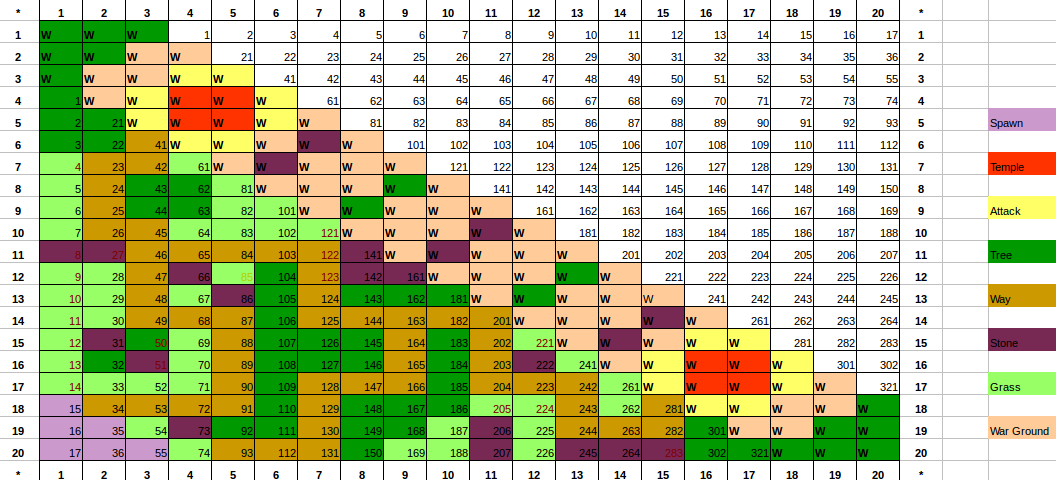
\includegraphics[width=1.1\textwidth]{Map_excel.png}
\caption{\label{fig:schematic}Schematic Map Representation}
\end{figure}


\section{Graphical Map Representation}
The graphical representation of our map respectively for both Demons and Angels is shown in Figure 3. Notice the visibility for both the teams. 

\begin{figure}[htp]
\centering
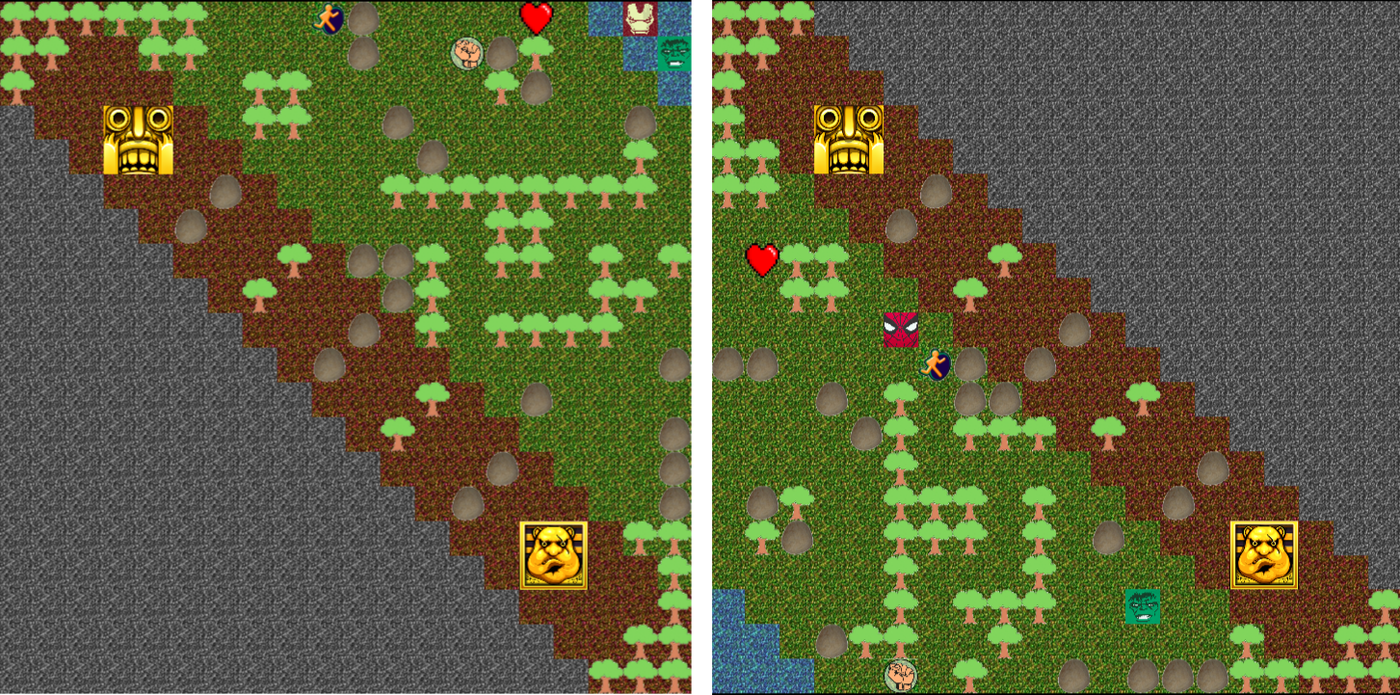
\includegraphics[width=1.0\textwidth]{Map_Views.png}
\caption{\label{fig:angels}Views of the Map}
\end{figure}


\section{Notification area}
The game is accompanied by an attribute area on both side of the maps, where the users can keep track of the game’s progress, etc. The schema for such an area is clearly depicted in Figure 4. 

\begin{figure}[htp]
\centering
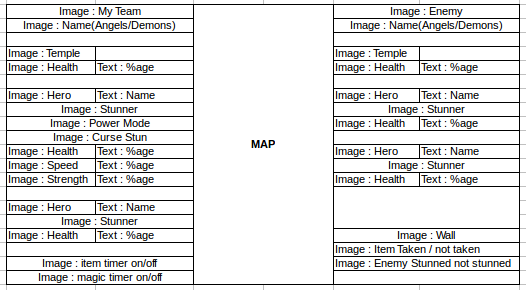
\includegraphics[width=0.9\textwidth]{attribute_space.png}
\caption{\label{fig:attribute}Schematic view of the attribute space}
\end{figure}


\section{Complete Map look}
The map in its entirety is shown in Figure 5. Notice the attribute area on either side.

\begin{figure}[htp]
\centering
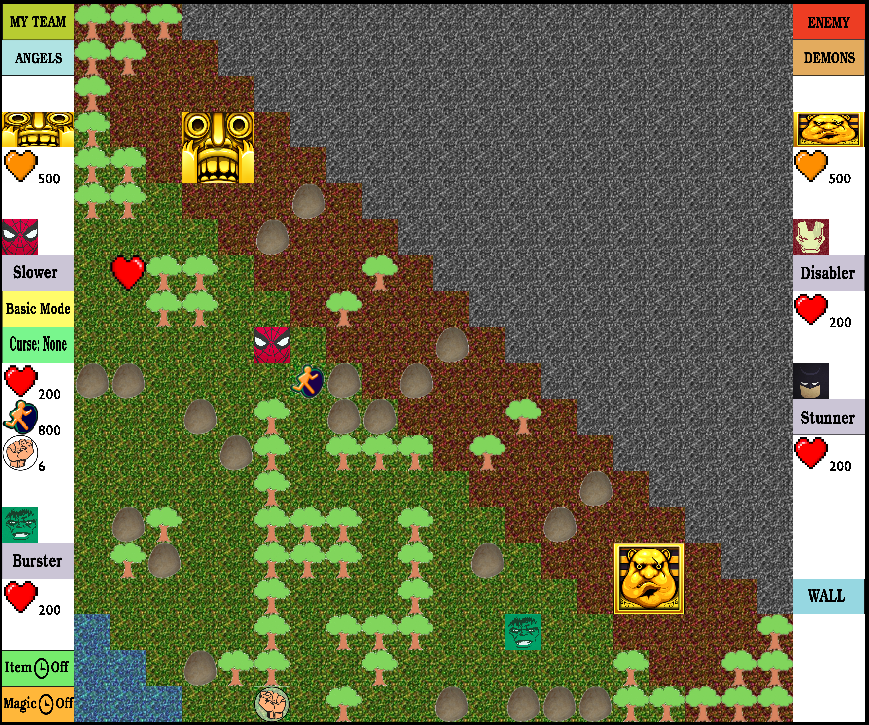
\includegraphics[width=0.7\textwidth]{Map_Attributes.png}
\caption{\label{fig:attributeMap}Complete Map with attribute space}
\end{figure}
